\documentclass{article}
\usepackage{amsmath,amssymb,amsthm, amsfonts}
\usepackage{color}
\usepackage{tikz}

\begin{document}

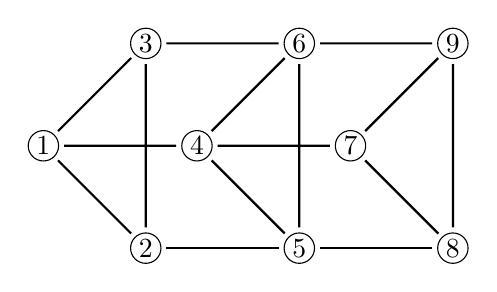
\begin{tikzpicture}[scale=1.3,every node/.style={draw,shape=circle,outer sep=2pt,inner sep=1pt,minimum size=.2cm}]		
\node[fill=none]  (1) at (-1,1) {$1$};
\node[fill=none]  (2) at (0,0) {$2$};
\node[fill=none]  (3) at (0,2) {$3$};
\node[fill=none]  (4) at (0.5,1) {$4$};
\node[fill=none]  (5) at (1.5,0) {$5$};
\node[fill=none]  (6) at (1.5,2) {$6$};
\node[fill=none]  (7) at (2,1) {$7$};
\node[fill=none]  (8) at (3,0) {$8$};
\node[fill=none]  (9) at (3,2) {$9$};
		
%Drawing the thick edges
\draw[thick] (1)--(2)--(3)--(1)--(4)--(5)--(6)--(4)--(7)--(8)--(9)--(7);
\draw[thick] (2)--(5)--(8);
\draw[thick] (3)--(6)--(9);
\end{tikzpicture}

\end{document}